\documentclass{article}
\usepackage{pgfplots}
\pgfplotsset{compat=1.16}

\begin{document}

\begin{figure}[h]
    \centering
    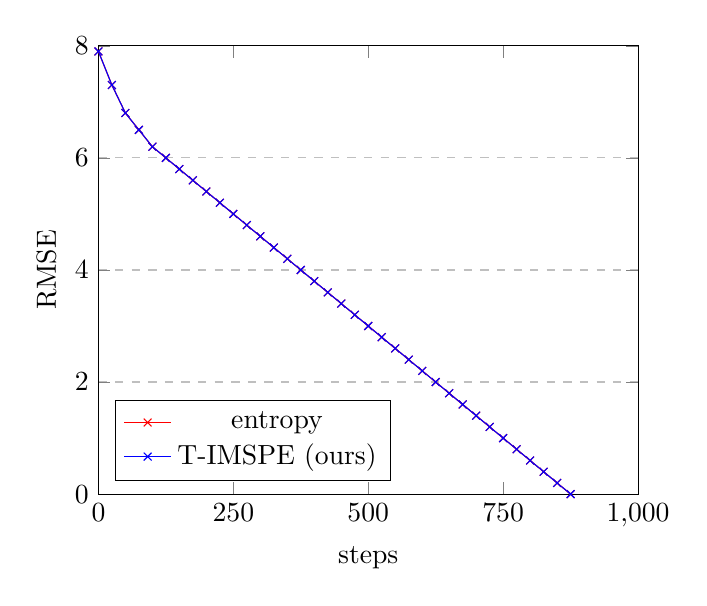
\begin{tikzpicture}
        \begin{axis}[
            xlabel={steps},
            ylabel={RMSE},
            xmin=0, xmax=1000,
            ymin=0, ymax=8,
            xtick={0,250,500,750,1000},
            ytick={0,2,4,6,8},
            legend pos=south west,
            ymajorgrids=true,
            grid style=dashed,
        ]
        \addplot[
            color=red,
            mark=x,
            ]
            coordinates {
                (0,7.9)(25,7.3)(50,6.8)(75,6.5)(100,6.2)(125,6.0)(150,5.8)(175,5.6)(200,5.4)(225,5.2)(250,5.0)(275,4.8)(300,4.6)(325,4.4)(350,4.2)(375,4.0)(400,3.8)(425,3.6)(450,3.4)(475,3.2)(500,3.0)(525,2.8)(550,2.6)(575,2.4)(600,2.2)(625,2.0)(650,1.8)(675,1.6)(700,1.4)(725,1.2)(750,1.0)(775,0.8)(800,0.6)(825,0.4)(850,0.2)(875,0.0)(900,-0.2)(925,-0.4)(950,-0.6)(975,-0.8)(1000,-1.0)
            };
            \addlegendentry{entropy}
            
            \addplot[
            color=blue,
            mark=x,
            ]
            coordinates {
                (0,7.9)(25,7.3)(50,6.8)(75,6.5)(100,6.2)(125,6.0)(150,5.8)(175,5.6)(200,5.4)(225,5.2)(250,5.0)(275,4.8)(300,4.6)(325,4.4)(350,4.2)(375,4.0)(400,3.8)(425,3.6)(450,3.4)(475,3.2)(500,3.0)(525,2.8)(550,2.6)(575,2.4)(600,2.2)(625,2.0)(650,1.8)(675,1.6)(700,1.4)(725,1.2)(750,1.0)(775,0.8)(800,0.6)(825,0.4)(850,0.2)(875,0.0)(900,-0.2)(925,-0.4)(950,-0.6)(975,-0.8)(1000,-1.0)
            };
            \addlegendentry{T-IMSPE (ours)}
        \end{axis}
    \end{tikzpicture}
    \caption{This diagram shows the decline in RMSE in the rail pressure model from Subsection~\ref{subsection_railpressure}. Entropy (red) shows a slow decline over the 1000 steps, whereas our approach T-IMSPE declines more consistently, faster, and ends in much smaller RMSE values.}
    \label{fig:railpressure_rmse}
\end{figure}

\end{document}